\chapter{Enquadramento Téorico}\label{ch:enquadramento}

A inteligência artificial é uma área da engenharia informática que se dedica ao desenvolvimento de algoritmos e sistemas capazes de simular a capacidade humana de raciocínio (e.g., aprendizagem, resolução de problemas, tomada de decisões).
De entre as várias aplicabilidades da inteligência artificial, destacam-se a visão computacional, o processamento de linguagem natural, a robótica e a aprendizagem automática (i.e., \textit{machine learning}.
No contexto da aprendizagem automática para o desenvolvimento de sistemas autónomos (i.e., que operam de forma independente, sem necessidade de intervenção externa, seja humana ou de outro sistema), a inteligência
Sendo que a autonomia é uma característica da inteligência,

A inteligência caracteriza-se pela relação entre a cognição (i.e. capacidade de realizar a ação adequada dadas as condições do ambiente) e a racionalidade (i.e., capacidade de decidir no sentido de conseguir o melhor resultado possível perante os objectivos que se pretende atingir

ser autónomo não significa ser inteligente, no entanto, a inteligência implica autonomia.


\section{Sistema Autónomo Inteligente}
O modelo de um sistema autónomo inteligente, também conhecido como agente inteligente, é uma abstracção que permite representar a interacção de um sistema com o seu ambiente. Este implementa um ciclo realimentado percepção-processamento-acção, através do qual é realizado o controlo da função do sistema de modo a concretizar a finalidade desse sistema (e.g., a travagem automática de um automóvel).

\begin{figure}[h]
    \begin{center}
        \resizebox{100mm}{!}{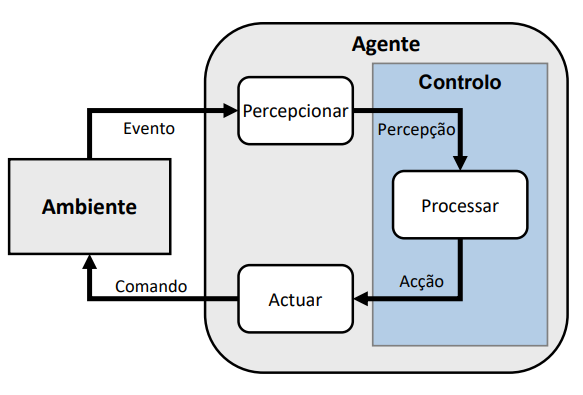
\includegraphics{../figures/modelo-agente-ambiente}}
    \end{center}
    \caption{Representação conceptual da
    relação entre agente e ambiente.}\label{fig:modelo-agente-ambiente}

\section{Ambiente}

O espaço onde um agente opera é designado por ambiente e caracteriza-se pelas seguintes propriedades:

\begin{itemize}
    \item \textbf{Determinístico vs. Estocástico}: um ambiente é determinístico se o estado seguinte é unicamente determinado pelo estado actual e pela acção do agente; caso contrário, é estocástico. Mais ainda, dizemos que um ambiente continua a ser determinístico, mas mais concretamente estratégico, caso estejamos num ambiente multi-agente onde o próximo estado pode estar também dependente das ações de outros agentes (e.g., num jogo de xadrez);
    \item \textbf{Episódico vs. Sequencial}: um ambiente é episódico se a experiência do agente é dividida em episódios independentes; caso contrário, é sequencial;
    \item \textbf{Estático vs. Dinâmico}: um ambiente é estático se não se altera enquanto o agente está a tomar uma decisão; caso contrário, é dinâmico;
    \item \textbf{Discreto vs. Contínuo}: um ambiente é discreto se o número de estados possíveis é finito; caso contrário, é contínuo;
    \item \textbf{Conhecido vs. Desconhecido}: um ambiente é conhecido se o agente tem acesso a uma descrição completa do ambiente; caso contrário, é desconhecido;
    \item \textbf{Tipo de Agente}: Os ambientes podem ser de agente único (i.e., apenas existe um agente a atuar) ou multi-agente (i.e., existem vários agentes a atuar, iguais ou diferentes).
\end{itemize}

A figura~\ref{fig:ambientes-exemplos} apresenta exemplos de ambientes com os atributos mencionados.

\begin{figure}[h]
    \begin{center}
        \resizebox{100mm}{!}{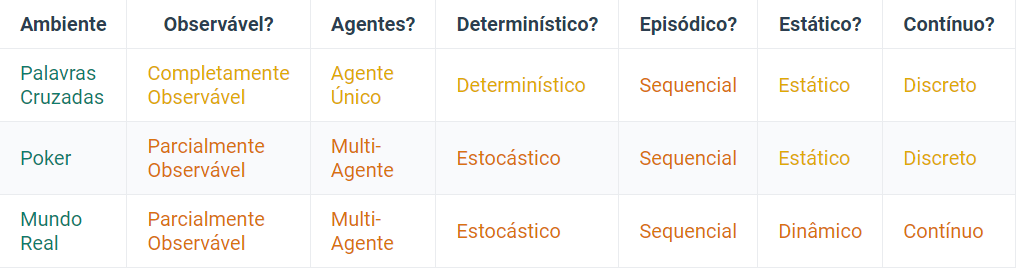
\includegraphics{../figures/ambientes-exemplos}}
    \end{center}
    \caption{Exemplos de ambientes com diferentes atributos.}\label{fig:ambientes-exemplos}
\end{figure}


\section{Agente Relacional}

Um agente racional é um tipo de agente que realiza as ações corretas, ou seja, deve conseguir, a partir da exploração e aprendizagem, descobrir estratégias para chegar ao seu objetivo de forma ótima.
Para esse efeito, é escolhida a ação que maximiza o valor esperado da medida de desempenho segundo a informação que lhes é fornecida (i.e., percepções) e o conhecimento adquirido até ao momento (e.g., conhecimento disponível sobre o ambiente).

\textbf{TODO: Rever/perg ao prof}

O conceito de recolha de informação entra neste contexto, visto que a exploração pode ser feita fora do âmbito do objetivo com vista
a adquirir conhecimento (e.g., estado do ambiente, ações possíveis, recompensas associadas a cada ação, etc) e, assim, melhorar a tomada de decisão seguinte.

No entanto, a ação tomada pode não resultar no que pretendemos

**Importante: a ação tomada pode não resultar no que pretendemos, visto que o raciocínio nem sempre leva ao sucesso**


\section{Arquiteturas de Agente}
\lipsum[1-2]

